\documentclass[border=10pt]{standalone}
\usepackage{tikz}\usepackage{amsmath}\usetikzlibrary{arrows.meta}
\begin{document}
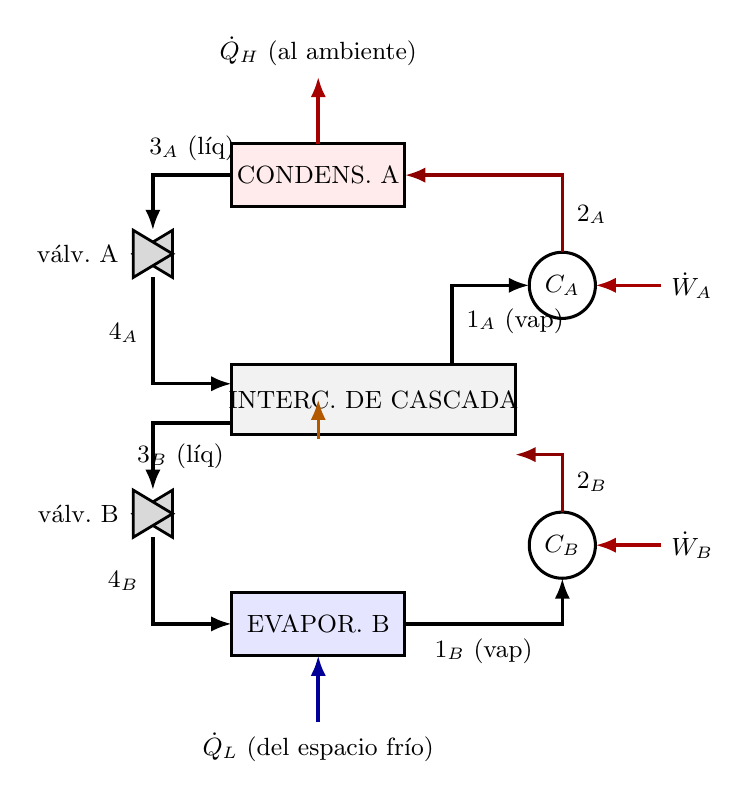
\begin{tikzpicture}[line width=1pt,>={Latex[length=2.6mm]}]
  % ============ INTERCAMBIADOR DE CASCADA (centro) ============
  \fill[black!5] (2.0,2.6) rectangle (5.6,3.5); \draw[line width=1.1pt] (2.0,2.6) rectangle (5.6,3.5);
  \node at (3.8,3.05){\small INTERC.\ DE CASCADA};
  % ============ CICLO SUPERIOR A (arriba) ============
  % condensador A
  \fill[red!8] (2.0,5.5) rectangle (4.2,6.3); \draw[line width=1.1pt] (2.0,5.5) rectangle (4.2,6.3);
  \node at (3.1,5.9){\small CONDENS.\ A};
  % compresor A
  \draw[line width=1.1pt] (6.2,4.5) circle (0.42); \node at (6.2,4.5){\small $C_A$};
  % valvula A
  \fill[black!15] (0.75,4.9)--(1.25,5.2)--(1.25,4.6)--cycle; \draw[line width=1.0pt] (0.75,4.9)--(1.25,5.2)--(1.25,4.6)--cycle;
  \fill[black!15] (1.25,4.9)--(0.75,5.2)--(0.75,4.6)--cycle; \draw[line width=1.0pt] (1.25,4.9)--(0.75,5.2)--(0.75,4.6)--cycle;
  \node[left] at (0.7,4.9){\small válv.\ A};
  % ============ CICLO INFERIOR B (abajo) ============
  % evaporador B
  \fill[blue!10] (2.0,-0.2) rectangle (4.2,0.6); \draw[line width=1.1pt] (2.0,-0.2) rectangle (4.2,0.6);
  \node at (3.1,0.2){\small EVAPOR.\ B};
  % compresor B
  \draw[line width=1.1pt] (6.2,1.2) circle (0.42); \node at (6.2,1.2){\small $C_B$};
  % valvula B
  \fill[black!15] (0.75,1.6)--(1.25,1.9)--(1.25,1.3)--cycle; \draw[line width=1.0pt] (0.75,1.6)--(1.25,1.9)--(1.25,1.3)--cycle;
  \fill[black!15] (1.25,1.6)--(0.75,1.9)--(0.75,1.3)--cycle; \draw[line width=1.0pt] (1.25,1.6)--(0.75,1.9)--(0.75,1.3)--cycle;
  \node[left] at (0.7,1.6){\small válv.\ B};
  % ---------- tuberias ciclo B (inferior) ----------
  \draw[->,line width=1.2pt] (4.2,0.2)--(6.2,0.2)--(6.2,0.78); \node[below] at (5.2,0.15){\small $1_B$ (vap)};
  \draw[->,red!55!black,line width=1.2pt] (6.2,1.62)--(6.2,2.35)--(5.6,2.35); \node[right] at (6.25,2.0){\small $2_B$};
  \draw[->,line width=1.2pt] (2.0,2.75)--(1.0,2.75)--(1.0,1.9); \node[below] at (1.35,2.62){\small $3_B$ (líq)};
  \draw[->,line width=1.2pt] (1.0,1.3)--(1.0,0.2)--(2.0,0.2); \node[left] at (0.95,0.75){\small $4_B$};
  % ---------- tuberias ciclo A (superior) ----------
  \draw[->,line width=1.2pt] (4.8,3.5)--(4.8,4.5)--(5.78,4.5); \node[right] at (4.85,4.05){\small $1_A$ (vap)};
  \draw[->,red!55!black,line width=1.2pt] (6.2,4.92)--(6.2,5.9)--(4.2,5.9); \node[right] at (6.25,5.4){\small $2_A$};
  \draw[->,line width=1.2pt] (2.0,5.9)--(1.0,5.9)--(1.0,5.2); \node[above] at (1.5,5.95){\small $3_A$ (líq)};
  \draw[->,line width=1.2pt] (1.0,4.6)--(1.0,3.25)--(2.0,3.25); \node[left] at (0.95,3.9){\small $4_A$};
  % ---------- interacciones ----------
  \draw[->,red!65!black,line width=1.3pt] (3.1,6.3)--(3.1,7.15); \node[above] at (3.1,7.15){\small $\dot Q_H$ (al ambiente)};
  \draw[->,blue!60!black,line width=1.3pt] (3.1,-1.05)--(3.1,-0.2); \node[below] at (3.1,-1.05){\small $\dot Q_L$ (del espacio frío)};
  \draw[<-,red!65!black,line width=1.3pt] (6.62,4.5)--(7.45,4.5); \node[right] at (7.45,4.5){\small $\dot W_A$};
  \draw[<-,red!65!black,line width=1.3pt] (6.62,1.2)--(7.45,1.2); \node[right] at (7.45,1.2){\small $\dot W_B$};
  % flecha de calor interno (B cede -> A absorbe)
  \draw[->,orange!70!black,line width=1.1pt] (3.1,2.55)--(3.1,3.05);
\end{tikzpicture}
\end{document}
